\chapter{Our Work}
\label{chap:prelim-exp}

\section{Overview}
This work presents a method dealing with challenges where we have a fully annotated dataset, however very small in size, and a large dataset but weakly annotated. We aim to overcome these challenges by implementing a hybrid approach for semantic segmentation of lymphocyte cells. Firstly, we try to train and validate a model on the small dataset itself. Then we use preprocessing and computer vision techniques to generate various pseudo-mask sets out of bounding-box annotations for the weakly annotated dataset and train a model on it, which is again validated on the small, fully annotated dataset. Then we try to identify and select the best fusing strategy for the mask sets, in order to utilize different abilities of the sets to capture the cell region. Next, we select the best model (with the most successful mask fusing strategy) and fine-tune it using a portion of data in the fully annotated dataset. We evaluate each of these experiments with Dice coefficient and IoU, and also create a confusion matrix for the final model, displaying which cell types were most confusing for it. We start with the fundamental part - the description of the datasets used.

\section{Datasets}
\label{sec:datasets}

\paragraph{TIGER} In our work, we use the TIGER dataset, which was released with the challenge under the same name on the Grand Challenge platform \cite{tiger_dataset}. It contains H\&E stained WSIs of Her2 positive and TNBC breast cancer tissues obtained by core needle biopsies or surgical resections. The images were scanned using 20x magnification. The dataset is released in three formats. We work with the one called WSIROIS. The WSIs come from three different institutions:

\begin{enumerate}
    \item TCGA (151 WSIs) dataset, contains images of TNBC from the TCGA-BRCA archive, annotations and magnification were adopted to be in line with those used further.
    \item RUMC (26 WSIs) images of both TNBC and Her2 positive breast cancer obtained from Radboud University Medical Center in the Netherlands, annotated by a panel of board-certified pathologists.
    \item JB (18 WSIs) images of both TNBC and Her2 positive breast cancer obtained from Jules Bordet Institute in Belgium, annotated by a panel of board-certified pathologists.
\end{enumerate}

The RUMC and JB WSIs contain 3 annotated ROIs with a size of approximately $500\!\times\!500$ \textmu m. The WSIs obtained from TCGA are more specific. This dataset was created by merging two other datasets: the BCSS (151 WSIs) and the NuCLS (124 WSIs). The NuCLS is a subset of the BCSS dataset. In the BCSS dataset, the tissue in a single large ROI is annotated but no cells are annotated. In the NuCLS a variable number of smaller ROIs are selected within the large ROI (same large ROI as in the BCSS) and these are densely annotated for multiple cell types. Annotations are adapted to match the other used annotations, as was mentioned.

The WSIROIS format contains:

\begin{itemize}
    \item WSI level annotations, wherein each WSI contains manual annotations of ROIs. Different tissue types are annotated with polygons, namely: invasive tumor, tumor-associated stroma, in-situ tumor, healthy glands, necrosis not in-situ, inflamed stroma, and rest. Most ROIs have also annotated plasma cells and lymphocytes. These were annotated using point annotations and then a bounding box was constructed and centered on the point of annotation with the size of $6\!\times\!6$ \textmu m, $8\!\times\!8$ \textmu m, or $9\!\times\!9$ \textmu m. Annotations for WSIs are released in XML format and also as a multi-resolution TIF image.
    \item ROI level annotations, where authors cropped the ROIs from WSIs and stored them as PNG files. Tissue type annotations are released as PNG images, containing pixel-level masks, and cell annotations are released in the COCO format - a JSON file containing file paths (the PNG images of ROIs) with IDs and metadata and corresponding annotations of bounding box position and size.
\end{itemize}

We further work with the part of the dataset that has ROI-level annotations. This part of the dataset consists of 1,879 (1,744 from TCGA, 81 from RUMC, 54 from JB) ROIs cropped from 44 (124 from TCGA, 26 from RUMC, 18 from JB). Together they contain 30,524 annotated cell nuclei.

An example of an image and its bounding box labels can be seen in Figure \ref{fig:tiger-with-without}.

\begin{figure}[H]
  \centering
  \begin{subfigure}[b]{0.32\textwidth}
    \centering
    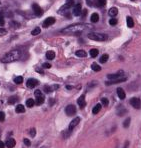
\includegraphics[width=\linewidth]{assets/images/for_presentation/image_TCGA-EW-A1P8-01Z-00-DX1.E9852193-8CDD-49EF-B49B-DA6931198F0D_[8391, 13690, 8532, 13838].png}
    \subcaption{Without annotations}\label{fig:tiger-img}
  \end{subfigure}%
  \quad
  \begin{subfigure}[b]{0.32\textwidth}
    \centering
    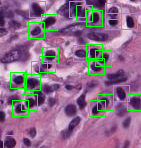
\includegraphics[width=\linewidth]{assets/images/for_presentation/bbox_TCGA-EW-A1P8-01Z-00-DX1.E9852193-8CDD-49EF-B49B-DA6931198F0D_[8391, 13690, 8532, 13838].png}
    \subcaption{With annotations}\label{fig:tiger-bbox}
  \end{subfigure}%
  \caption{Example of TIGER image without and with annotations of TILs \cite{tiger_dataset}}
  \label{fig:tiger-with-without}
\end{figure}

\paragraph{TNBC} Triple Negative Breast Cancer Nuclei Segmentation dataset \cite{TNBC-nuclei-seg}, is an open dataset consisting of 11 patients with breast cancer, with varying numbers of images for each patient, provided regions of interest (ROIs) PNGs. Together, it has 50 annotated ROIs of size 512x512, scanned with the 40x magnification. Specifically, we use the extended version of this dataset \cite{TNBC-nuclei-seg-extended}, where annotations of cell classes were added. Each image has a corresponding pixel mask, where each pixel is labeled by the class it represents. There are 11 different cell classes plus background and unknown class. We also note that this extended version of the dataset provides images of brain tissue, but since it is not part of our work, we only work with the images of breast cancer. An example image with its ground truth mask, already relabeled so only lymphocytes are annotated, can be seen in figure \ref{fig:tcga-with-without}.

\begin{figure}[H]
  \centering
  \begin{subfigure}[b]{0.32\textwidth}
    \centering
    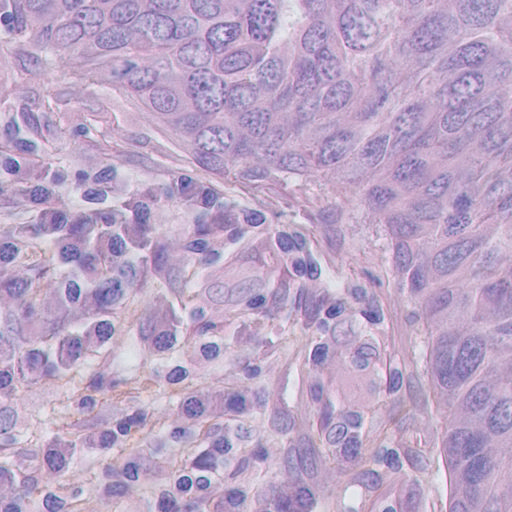
\includegraphics[width=\linewidth]{assets/images/for_presentation/image_10_1.png}
    \subcaption{Image}\label{fig:tcga-img}
  \end{subfigure}%
  \hfill
  \begin{subfigure}[b]{0.32\textwidth}
    \centering
    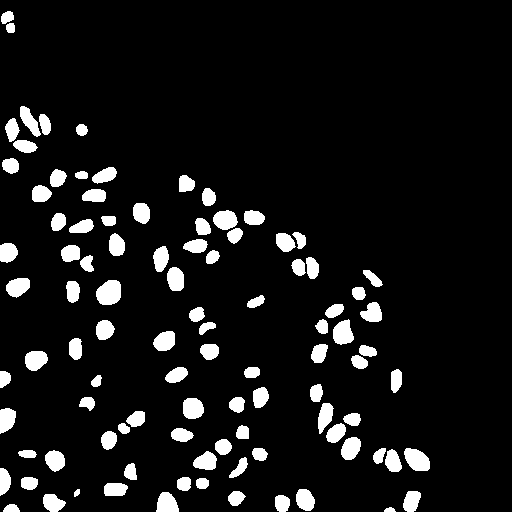
\includegraphics[width=\linewidth]{assets/images/for_presentation/mask_10_1.png}
    \subcaption{Mask}\label{fig:tcga-mask}
  \end{subfigure}%
  \hfill
  \begin{subfigure}[b]{0.32\textwidth}
    \centering
    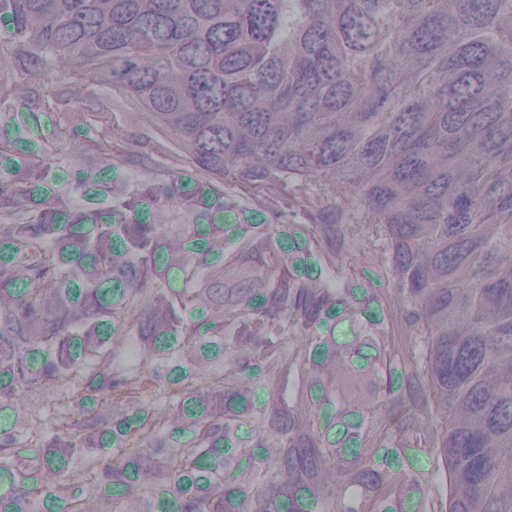
\includegraphics[width=\linewidth]{assets/images/for_presentation/overlay_10_1.png}
    \subcaption{Image with mask overlay}\label{fig:tcga-overlay}
  \end{subfigure}%
  \caption{Example of TNBC image, mask and overlay, where TILs are annotated \cite{TNBC-nuclei-seg-extended}}
  \label{fig:tcga-with-without}
\end{figure}

\section{Deep Learning Model}

\subsection{Architecture}
As a deep learning model for semantic segmentation, we employ the U-Net architecture. U-Net is a powerful architecture, and as we mention in Chapter \ref{chapter:dnn}, in Section \ref{chapter:dnn-section:arch}, it is also widely used in the medical imaging domain. Specifically, we use the ResNet-34 encoder as the U-Net's backbone, which is already pretrained on the ImageNet dataset. This choice was based on the fact that residual blocks further improve the U-Net's ability to learn, as we continue to write in Section \ref{chapter:dnn-section:arch} of Chapter \ref{chapter:dnn}. In the state-of-the-art, which we present in Chapter \ref{chapter:related}, authors in \cite{Zhang2022, Liang2023} also use ResNet architectures, and specifically, ResNet-34 is used in \cite{Lin2023}. The inspiration to initialize the encoder with weights pretrained on the ImageNet dataset came from the state-of-the-art works as well, where a similar approach was used in \cite{Zhang2022, Lin2023, Liang2023}. The full architecture of the model can be seen in Figure \ref{fig:our-architecture}.

\begin{figure}[H]
\begin{centering}
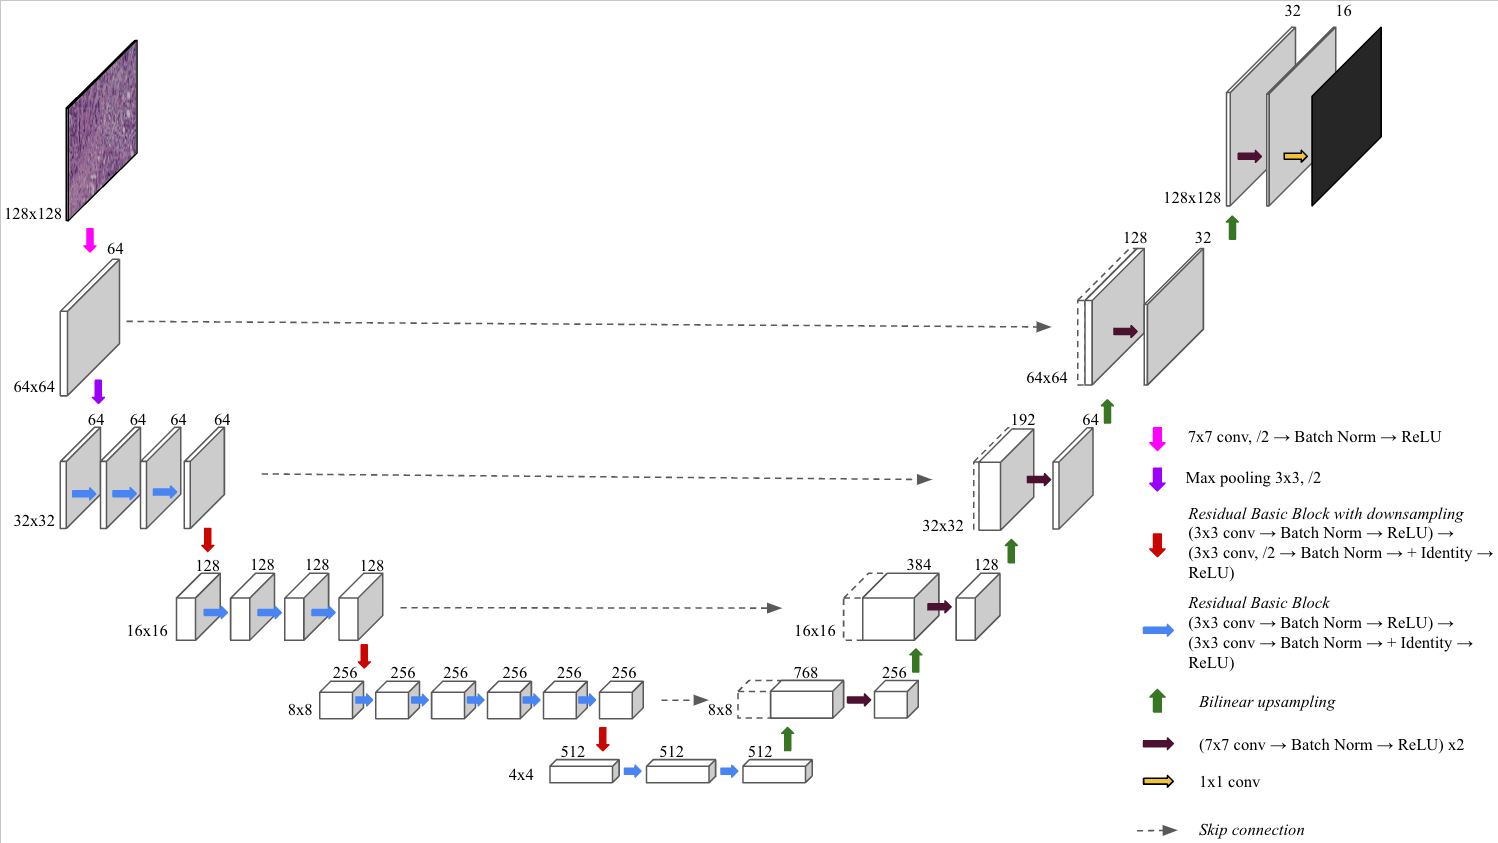
\includegraphics[width=\textwidth]{assets/images/for_presentation/our_architecture.png}
\par\end{centering}
\caption{The architecture of our model 
\label{fig:our-architecture}}
\end{figure}

This model is being used in all our experiments as the segmentation model. The training setup and model's hyperparameters remain the same in every experiment as well. 

\subsection{Input and Output Specifications}
The input for the model is an image of size $128\times128$ pixels in a 3 - RGB - channel space. The model's segmentation head produces a binary mask of size $128\times128$ pixels and a depth of 1. The output mask is then run through the sigmoid function, to squeeze the values between 0 and 1. A threshold of 0.5 is applied to this mask as pixels with a value less than 0.5 are predicted background and labeled with a number 0, and pixels with a value greater than or equal to 0.5 are predicted TILs and labeled with a number 1.

\subsection{Loss Function}
The loss function used during training is the Dice Loss function. This loss function is the preferred function to be used in the segmentation of objects and is also frequently used in the medical imaging domain, as described in \cite{Zhang2021}.

\subsection{Optimization}
We used the Adam optimizer, and the initial learning rate was set to 0.001, and it was reduced every 5 epochs by a factor of 0.1. Early stopping was also used, where the patience was set to 10 epochs - if the validation loss was not improved over the 10 epochs, the training stopped to prevent overfitting.

\subsection{Training}
Every training was set to run for 100 epochs, if it was not stopped earlier. The batch size was set to 16 samples. Checkpoints of the model were periodically saved every epoch - always the best checkpoint (in terms of validation loss). If CUDA framework was available, the training run on the GPU, if not then on the CPU. During the training stage, we monitored the model's performance on various variables. These included accuracy, recall, precision, Dice coefficient, IoU, and the running loss.

For the training purpose, we further split the training data into the training subset (80\% of the whole training dataset) and the validation subset (20\% of the whole training dataset). Then in each epoch, we let the model process the whole training subset (in the form of batches), while monitoring and logging the aforementioned variables. After each epoch, we set the model into the validation mode. In this mode, the model does not update its parameters. We let it process the validation subset and also monitor and log the variables, out of which the most interesting for us is the validation loss, since this is used both for the early stopping and for saving the checkpoints. After the validation was completed, we set the model into the training mode again, where it could further update its parameters. This whole process was repeated until the training was finished, and the model could be evaluated on the testing dataset.

\section{Evaluation Methods}
Upon completing the training process, we initiated the final evaluation of the segmentation model. The best-performing model, determined by the lowest validation loss, was loaded from the saved checkpoint and set to evaluation mode to prevent any parameter updates. Subsequently, the model processed the entire testing dataset, and the final testing metrics were computed.

We assessed the model using both quantitative and qualitative methods. The quantitative evaluation included the Dice coefficient and IoU metrics - we describe these in more detail and why they are most suitable for segmentation tasks in Chapter \ref{chapter:dnn}, in Section \ref{chapter:dnn:eval}. For qualitative assessment, we visualized the predicted binary masks alongside the ground truth masks to facilitate direct comparison.

\section{Data Preprocessing}
Since we work with two very distinct datasets, and furthermore, the TIGER dataset is composed of three other datasets, we need to employ a robust preprocessing framework in order to align all datasets on the same level.

\subsection{Normalization} 
TIGER and TNBC datasets pose several challenges to us. Firstly, as we described in section \ref{sec:datasets}, data come from four distinct sources (three for TIGER and one for TNBC) - this means that the staining is very different, which we can see in Figure \ref{fig:mix-no-norm}.

% Image
\begin{figure}[H]
  \centering
  % First row (2 images)
  \begin{subfigure}[b]{0.32\textwidth}
    \centering
    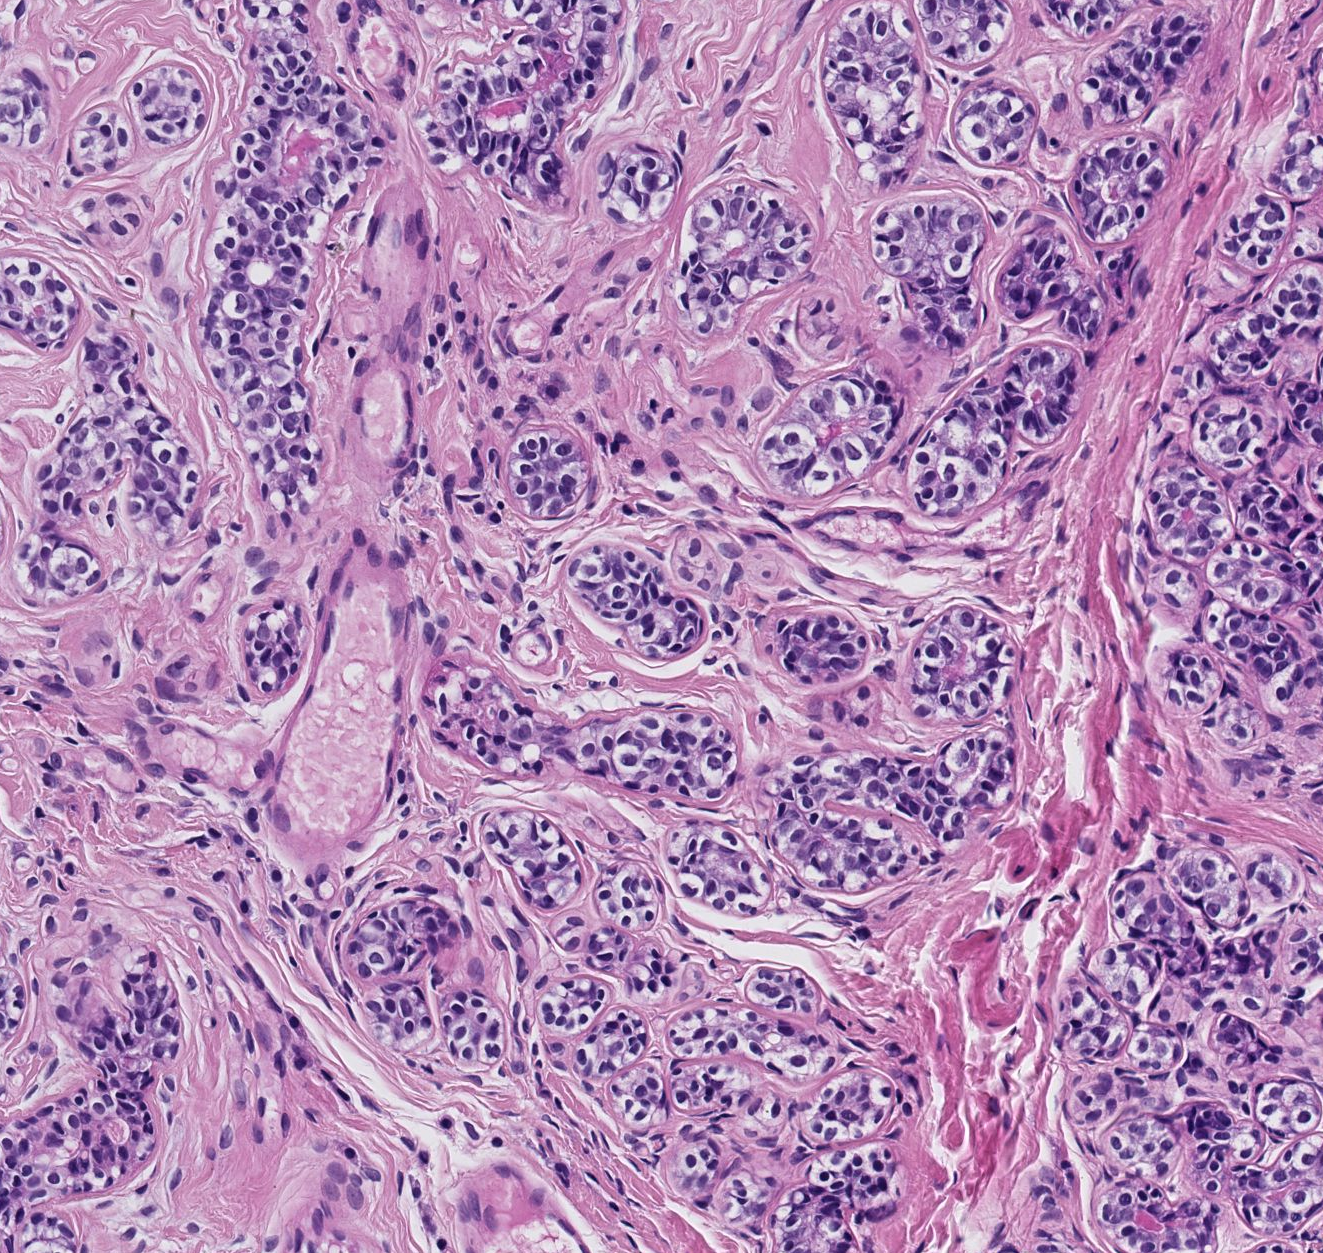
\includegraphics[width=\linewidth]{assets/images/for_presentation/image_100B_[10779, 11621, 12102, 12874].png}
    \caption{TIGER image – JB}
  \end{subfigure}\quad
  \begin{subfigure}[b]{0.32\textwidth}
    \centering
    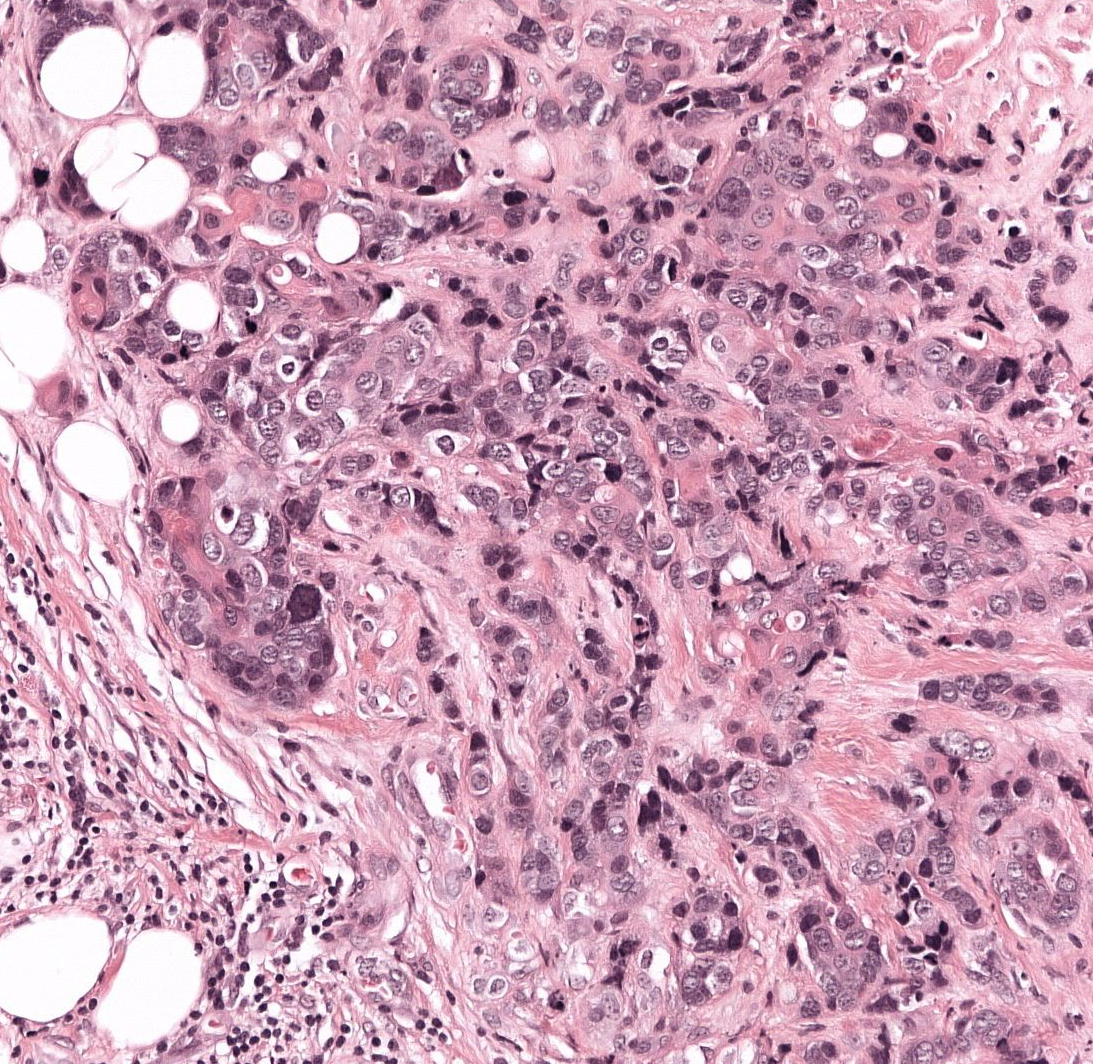
\includegraphics[width=\linewidth]{assets/images/for_presentation/image_TC_S01_P000003_C0001_B104_[50106, 52730, 51199, 53794].png}
    \caption{TIGER image – TC}
  \end{subfigure}

  \par\vspace{1em} % line break with a little vertical space

  % Second row (2 images)
  \begin{subfigure}[b]{0.32\textwidth}
    \centering
    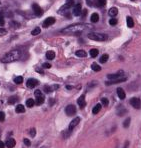
\includegraphics[width=\linewidth]{assets/images/for_presentation/image_TCGA-EW-A1P8-01Z-00-DX1.E9852193-8CDD-49EF-B49B-DA6931198F0D_[8391, 13690, 8532, 13838].png}
    \caption{TIGER image – TCGA}
  \end{subfigure}\quad
  \begin{subfigure}[b]{0.32\textwidth}
    \centering
    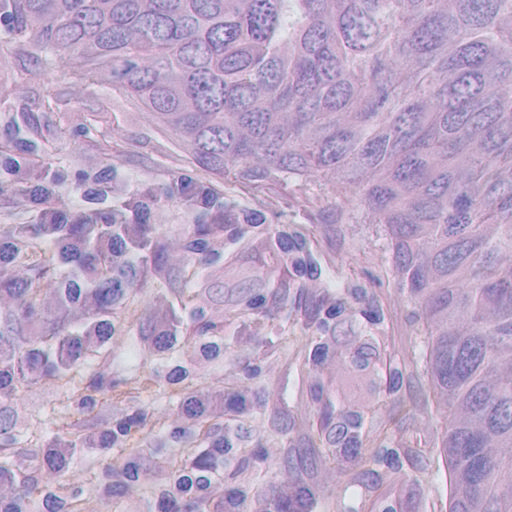
\includegraphics[width=\linewidth]{assets/images/for_presentation/image_10_1.png}
    \caption{TNBC image}
  \end{subfigure}

  \caption{Example images from TIGER datasets \cite{tiger_dataset} and TNBC \cite{TNBC-nuclei-seg-extended} before normalization.}
  \label{fig:mix-no-norm}
\end{figure}

We employ the multi-target Macenko stain normalization technique as described in \cite{Ivanov2024}, where we select 8 reference images from the TIGER and 2 reference images from the TNBC dataset. This number is arbitrary, but in \cite{Ivanov2024} authors experimented with a different number of reference images (2-20) and showed that the higher number has slightly better results, but if the number is too high, there are no significant improvements. Given the sizes of our respective datasets, we decided to go with the 8 and 2 images. Then we used the same 10 reference images to normalize both datasets. The normalization technique improved the color inconsistencies, as we can see in Figure \ref{fig:mix-norm}.

\begin{figure}[H]
  \centering
  % First row (2 images)
  \begin{subfigure}[b]{0.32\textwidth}
    \centering
    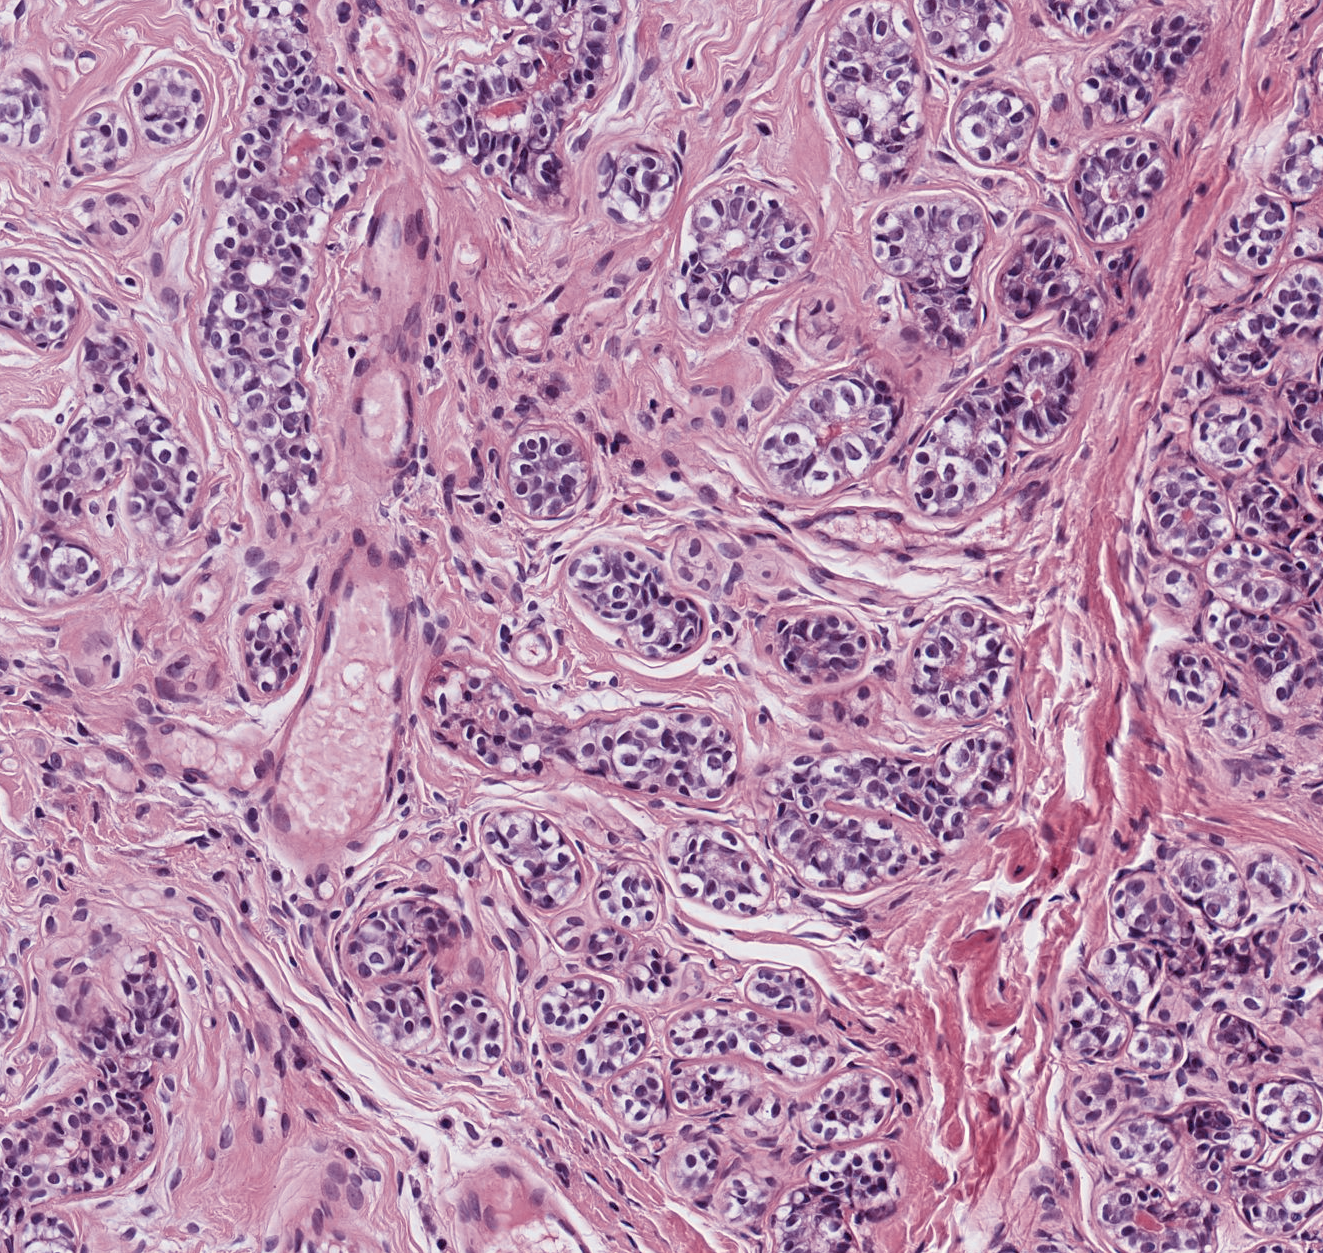
\includegraphics[width=\linewidth]{assets/images/for_presentation/norm_100B_[10779, 11621, 12102, 12874].png}
    \caption{TIGER image – JB}
  \end{subfigure}\quad
  \begin{subfigure}[b]{0.32\textwidth}
    \centering
    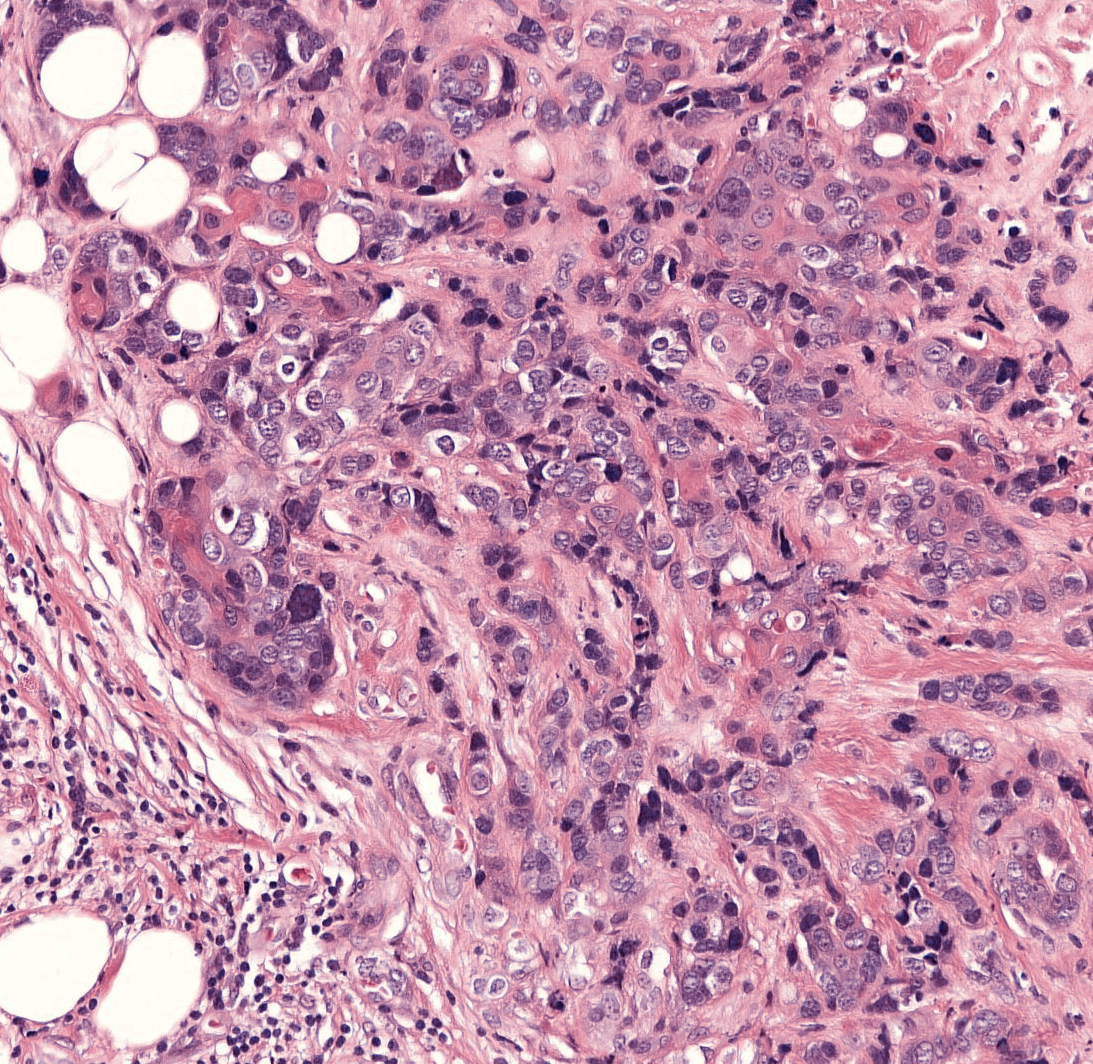
\includegraphics[width=\linewidth]{assets/images/for_presentation/norm_TC_S01_P000003_C0001_B104_[50106, 52730, 51199, 53794].png}
    \caption{TIGER image – TC}
  \end{subfigure}

  \par\vspace{1em} % line break with a little vertical space

  % Second row (2 images)
  \begin{subfigure}[b]{0.32\textwidth}
    \centering
    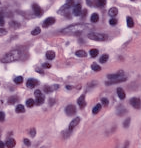
\includegraphics[width=\linewidth]{assets/images/for_presentation/norm_TCGA-EW-A1P8-01Z-00-DX1.E9852193-8CDD-49EF-B49B-DA6931198F0D_[8391, 13690, 8532, 13838].png}
    \caption{TIGER image – TCGA}
  \end{subfigure}\quad
  \begin{subfigure}[b]{0.32\textwidth}
    \centering
    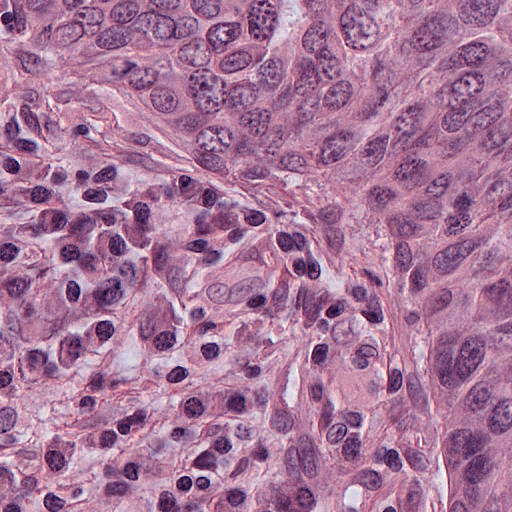
\includegraphics[width=\linewidth]{assets/images/for_presentation/norm_10_1.png}
    \caption{TNBC image}
  \end{subfigure}

  \caption{Example images from TIGER datasets \cite{tiger_dataset} and TNBC \cite{TNBC-nuclei-seg-extended} after normalization.}
  \label{fig:mix-norm}
\end{figure}

% Image

\subsection{Pseudo-mask sources} 
\label{subs:mask-sources}
The next step was to generate the pseudo-masks. For this, we created different variations of the same image. We named the images that were created as a part of one variation \textit{image source}. In total, six different image sources were created for the experiments. We used the original (raw) image as one source, then the normalized image as another source. Furthermore, we extracted the hematoxylin image out of the original image (Macenko normalization does this internally). This was done based on the fact that hematoxylin highlights the cell nuclei, as we described in Chapter \ref{chapter:intro}. This hematoxylin image became our third image source. Lastly, by applying histogram equalization to all of the aforementioned image sources (to increase the overall contrast of the image and shift dark colors into darker ones and light into lighter ones), we obtained another three image sources. The difference in the image sources can be seen in Figure \ref{fig:tiger-sources}. 

\begin{figure}[H]
  \centering
  % First row of three subfigures
  \begin{subfigure}[b]{0.32\textwidth}
    \centering
    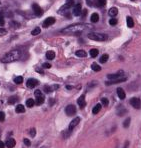
\includegraphics[width=\linewidth]{assets/images/for_presentation/image_TCGA-EW-A1P8-01Z-00-DX1.E9852193-8CDD-49EF-B49B-DA6931198F0D_[8391, 13690, 8532, 13838].png}
    \caption{Original image}\label{fig:tiger-raw}
  \end{subfigure}\hfill
  \begin{subfigure}[b]{0.32\textwidth}
    \centering
    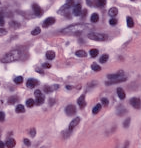
\includegraphics[width=\linewidth]{assets/images/for_presentation/norm_TCGA-EW-A1P8-01Z-00-DX1.E9852193-8CDD-49EF-B49B-DA6931198F0D_[8391, 13690, 8532, 13838].png}
    \caption{Normalized image}\label{fig:tiger-norm}
  \end{subfigure}\hfill
  \begin{subfigure}[b]{0.32\textwidth}
    \centering
    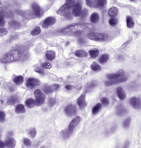
\includegraphics[width=\linewidth]{assets/images/for_presentation/hem_TCGA-EW-A1P8-01Z-00-DX1.E9852193-8CDD-49EF-B49B-DA6931198F0D_[8391, 13690, 8532, 13838].png}
    \caption{Hematoxylin image}\label{fig:tiger-hem}
  \end{subfigure}

  % Line break to start the second row; adjust vertical space as needed
  \par\vspace{1em}

  % Second row of three subfigures
  \begin{subfigure}[b]{0.32\textwidth}
    \centering
    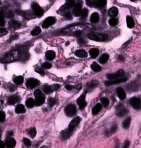
\includegraphics[width=\linewidth]{assets/images/for_presentation/eq_TCGA-EW-A1P8-01Z-00-DX1.E9852193-8CDD-49EF-B49B-DA6931198F0D_[8391, 13690, 8532, 13838].png}
    \caption{Original image with histogram equalization}\label{fig:tiger-eq}
  \end{subfigure}\hfill
  \begin{subfigure}[b]{0.32\textwidth}
    \centering
    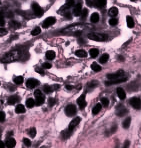
\includegraphics[width=\linewidth]{assets/images/for_presentation/norm_eq_TCGA-EW-A1P8-01Z-00-DX1.E9852193-8CDD-49EF-B49B-DA6931198F0D_[8391, 13690, 8532, 13838].png}
    \caption{Normalized image with histogram equalization}\label{fig:tiger-norm-eq}
  \end{subfigure}\hfill
  \begin{subfigure}[b]{0.32\textwidth}
    \centering
    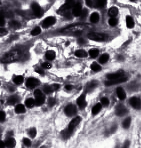
\includegraphics[width=\linewidth]{assets/images/for_presentation/hem_eq_TCGA-EW-A1P8-01Z-00-DX1.E9852193-8CDD-49EF-B49B-DA6931198F0D_[8391, 13690, 8532, 13838].png}
    \caption{Hematoxylin image with histogram equalization}\label{fig:tiger-hem-eq}
  \end{subfigure}
  \caption{Examples of image sources}
  \label{fig:tiger-sources}
\end{figure}


We then operated on each image source with different computer vision techniques to generate the final pseudo-mask PNGs. We describe each of these techniques in the section \ref{section:mask-generation}. 

\subsection{Aligning the TNBC dataset} 
In order to use the \\ 
TNBC dataset, we needed to align its scale and also the ground truth masks. This dataset was scanned with the $40\times$ magnification; however, the TIGER dataset was scanned using the $20\times$ magnification. To align them, we down-scaled the TNBC dataset images and masks by the factor of 2. Moreover, the 
\\ TNBC ground truth masks were relabeled to binary masks by setting all of the other labels except for the lymphocyte cell labels as background.

\subsection{Patching Strategy}
To be able to feed our data to the deep learning UNet model, we created patches of fixed size $128\times128$ pixels. The TIGER dataset contained images of varying sizes. Therefore, we created overlapping patches with dynamic stride in such a way, that no patch was shifted outside of the original image. We created 19,386 patches of TIGER dataset images. The TNBC dataset was nicer since the original images were of $512\times512$ pixels in size, and after down-scaling by a factor of 2, they became $256\times256$ pixels. Each image was then split into 4 non-overlapping patches. This got us exactly 200 patches of TNBC dataset images. After this stage, the data is ready for the training and evaluation process.

\subsection{Images to Tensors}
For the PyTorch framework to work with the PNG image patches, both original images and masks, we needed to convert them from NumPy arrays into tensors. This was done before the training and evaluation of each trained model.

\section{Pseudo-masks Generation}
\label{section:mask-generation}
To be able to start a training of our segmentation model on the TIGER dataset, we needed to convert the bounding box annotations of lymphocyte nuclei into pixel-level pseudo-masks. We used a series of computer vision methods, which were chained in different ways in order to better identify the region where a cell nuclei is present within the bounding box. This task was challenging because of the lower contrast between the nuclei and the surrounding tissue, and also because some nuclei were too close to each other, meaning that there was an overlap between the bounding boxes. This inspired us to create different versions of a single image, to promote some properties of the image, such as increasing the contrast, or isolating only the hematoxylin staining. We called these versions image sources and the process of their creation is described in Subsection \ref{subs:mask-sources} as a part of image preprocessing. The whole process of pseudo-mask generation can be seen in Figure \ref{fig:dg-mask-gen}. To better understand the chain of operations applied, we will illustrate it on a single image example of one image source:

\begin{enumerate}
    \item Firstly the image is loaded together with its corresponding bounding box annotations.
    \item Next, the individual labeled nuclei are cropped out of the image, using the bounding box values.
    \item Then a four combinations of operations are applied on the cropped region, which means that from the single cropped region, four new versions of it are created, based on which combination of operations was applied. It was either:
    \begin{itemize}
        \item The Otsu thresholding
        \item The Adaptive thresholding
        \item The median blur with Otsu thresholding
        \item The median blur Adaptive thresholding
    \end{itemize}
    \item In the next step the morphological opening is applied to remove small artifacts left after the thresholding.
    \item The previous operations created so far a 'prototype' of the pseudo-mask. In the subsequent step, the marked watershed is applied, which use this prototype together with the initial cropped image region to create a final pseudo-mask.
    \item Finally, the small pseudo-masks for individual cells are combined into a full-patch pseudo-mask
\end{enumerate}

\begin{figure}[H]
\begin{centering}
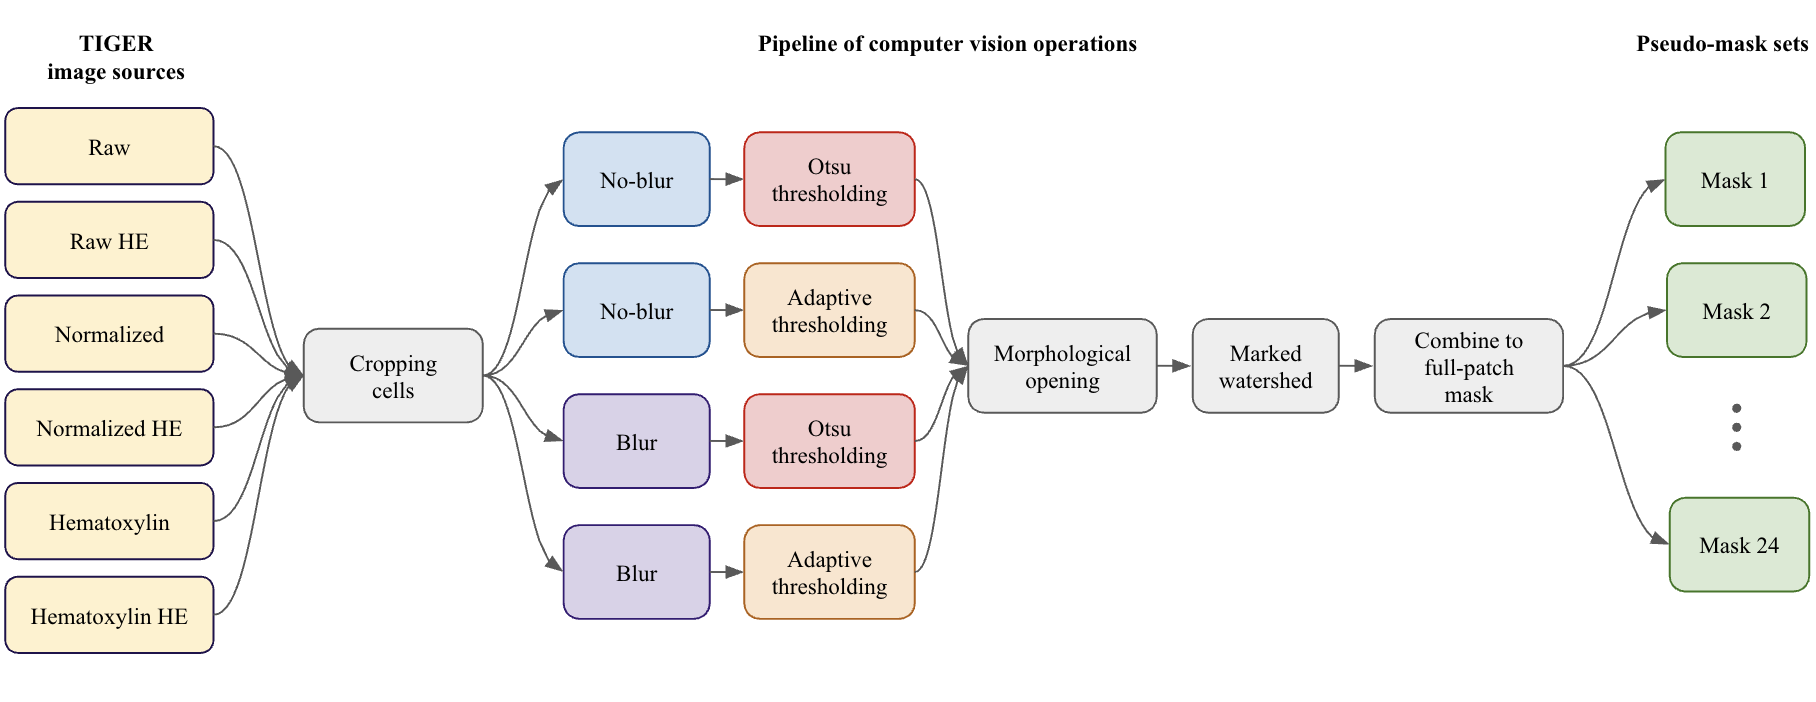
\includegraphics[width=\textwidth]{assets/images/for_presentation/dg-mask-gen.png}
\par\end{centering}
\caption{The process of pseudo-masks generation 
\label{fig:dg-mask-gen}}
\end{figure}

Given that we work with 6 image sources and 4 pipelines of computer vision operations, where each pipeline is applied to every image source, this gives us in total 24 pseudo-masks for any given image. In the below paragraphs, we describe each computer vision operation in more detail.

\paragraph{Median Blur}
We use the $3\times3$ median blur with the intuition that it could remove small noises around the cell nuclei. This filter replaces each pixel with the median of its neighborhood, which is determined by the size of the kernel. We use the kernel of size $3\times3$ - this is reasonable for us, since the bounding boxes are of size $12\times12$, $16\times16$, or $18\times18$ and we do want to remove possible small noise but still preserve the shape of the nuclei.

\paragraph{Otsu Thresholding}
The Otsu thresholding finds a threshold that minimizes intra-class variance and then binarizes the pixel values based on this threshold. Since this operation needs a grayscale image, we first do this conversion. Then we apply the Otsu thresholding method and inversion - this automatically computes the optimal Otsu threshold and also inverts the binarization so that dark nuclei appear as white foreground and background pixels become black.

\paragraph{Adaptive Thresholding}
In contrast to Otsu thresholding, adaptive thresholding computes the threshold for each pixel based on its neighborhood. We use the $11\times11$ adaptive thresholding with a constant of 2 - this ensures that we cover the small nuclei diameter but still preserve fine details. In the Equation \ref{eq:adaptive} we can see how the threshold $T(x,y)$ is computed for each pixel with coordinates $x$ and $y$. Firstly, a window $\mathcal{W}$ of size $B\times B$ is centered around the pixel. Then each pixel's grayscale intensity $I(u,v)$ within this window with pixel coordinates $u$ and $v$ is summed and then averaged. Finally, a constant is subtracted from this mean to bias the threshold below the local mean.

\begin{align}
\label{eq:adaptive}
T(x,y)
=
\frac{1}{B^2}
\sum_{u = x - \frac{B-1}{2}}^{\,x + \frac{B-1}{2}}
\;\;
\sum_{v = y - \frac{B-1}{2}}^{\,y + \frac{B-1}{2}}
I(u,v)
\;-\; C
\end{align}

\paragraph{Morphological Opening}
We use the elliptical $3\times3$ morphological opening to remove any small artifacts left after the thresholding operations and to preserve the shape of the nuclei.

\paragraph{Marked Watershed}
To obtain the final pseudo-mask, we employ the mark-controlled watershed. This includes a series of steps:
\begin{enumerate}
    \item Firstly, the distance transform operation computes, for each foreground pixel in the so-far-created binary mask, the Euclidean distance to the nearest background pixel, producing a map whose peaks lie at object centers.
    \item Secondly, we threshold the distance map, which keeps only the central ~30\% of each cell nuclei - this helps to separate the touching nuclei and gives us the pseudo-mask of sure foreground area (the sure nuclei area).
    \item Then we dilate the sure foreground with $3\times3$ elliptical kernel to expand the region. Now we consider all pixels lying outside of these regions as sure background.
    \item After that we subtract the sure foreground from the sure background mask. This gives us the regions that should have shape of ring and are 'unknown' - either background or foreground. Those are the pixels that lie on the boundaries of each cell.
    \item Next we do marker labeling - we mark each connected component of the sure foreground mask with different mark (integer), starting with number 1. Then we add number 1 to each pixel value. Lastly, we set those pixels which are marked as unknown region to zero. This step ensures that:
    \begin{itemize}
        \item The sure foreground areas start from number 2 onward,
        \item The sure background areas are marked with number 1, and
        \item The unknown regions are marked with number 0.
    \end{itemize}
    \item Finally, the watershed algorithm will flood and try to segment the unknown regions (marked with 0). It treats the original image provided to it (the colorful crop of cell nuclei) as a height map, where the brighter pixels represents high elevations and the darker represents low elevations. It also uses the marker image to seed the foreground and background regions. During the segmentation process, it floods the image starting at each marker label and when the floods meet, the lines separating the cell nuclei are created. Pixels on these delineating lines have a value set to -1.
\end{enumerate}

After the mark-controlled watershed produces the delineated nuclei mask, we set all pixel values that are lower than or equal to 1 to 0 (sure background and delineation lines) and those that are greater than 1 (all nuclei components) to 1 to create a binary pseudo-mask.

\paragraph{Full-patch Combining}
After we obtain the small-sized pseudo-masks for each cell nuclei bounding box, we reconstruct the full-patch mask by firstly creating an image where all pixels have 0 values and then applying the binary OR operation with the small-sized pseudo-masks on the position from which they were cropped. By this, we get the final pseudo-mask for the original image, where pixels of nuclei regions have values of 1 and background pixels have values of 0.

\section{Pseudo-masks Fusion}
\label{section:mask-fusion}
During the generation of pseudo-masks, we obtained 24 different masks per single image. We decided to fuse them based on the results of experiment which we present in Subsection \ref{sub:exp-2} and based on the visualization of the combined masks, which we can see in Figure \ref{fig:combined-vis}. These combined masks were created using the pixel-wise addition of all 24 pseudo-masks, which gave us a single pseudo-mask per image, where pixel values ranged between 0 (all pseudo-masks labeled the pixel as background) and 24 (all masks labeled the pixel as foreground). For the purpose of visualization, a pixel-wise multiplication by number 10 was applied on the resulting pseudo-mask, to better see the combined power of the pseudo-mask.

\begin{figure}[H]
  \begin{subfigure}[b]{0.24\textwidth}
    \centering
    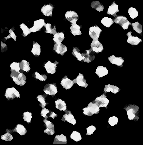
\includegraphics[width=\linewidth]{assets/images/for_presentation/combined-1.png}
  \end{subfigure}\hfill
  \begin{subfigure}[b]{0.24\textwidth}
    \centering
    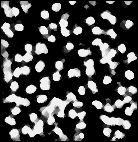
\includegraphics[width=\linewidth]{assets/images/for_presentation/combined-2.png}
  \end{subfigure}\hfill
  \begin{subfigure}[b]{0.24\textwidth}
    \centering
    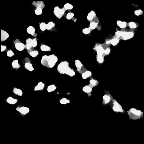
\includegraphics[width=\linewidth]{assets/images/for_presentation/combined-3.png}
  \end{subfigure}
  \begin{subfigure}[b]{0.24\textwidth}
    \centering
    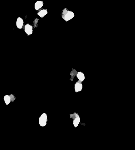
\includegraphics[width=\linewidth]{assets/images/for_presentation/combined-4.png}
  \end{subfigure}
  \caption{Examples of combined pseudo-masks}
  \label{fig:combined-vis}
\end{figure}

We decided to try two different fusion approaches:

\begin{enumerate}
  \item Fuse the pseudo-masks via pixel-wise voting at quartile agreement levels - 100\%, 75\%, 50\%, and 25\% - keeping only those pixels declared foreground by at least that percentage of the masks which achieved the highest Dice scores in the experiment of Subsection~\ref{sub:exp-2}. This gave us four sets of fused masks. The overview of this fusing approach can be seen in Figure \ref{fig:dg-mask-fuse-2}. Firstly, the masks are summed together (pixel-wise) and then all pixels that are greater than 0 are set to 1 (foreground - nuclei) to maintain the binary mask.
  \item Fuse the pseudo-masks via pixel-wise voting consensus by all involved masks - a pixel was labeled as foreground (cell nuclei) if either:
  \begin{itemize}
      \item 24 out of 24 masks declared the pixel as foreground,
      \item 23 out of 24 masks declared the pixel as foreground,
      \item 22 out of 24 masks declared the pixel as foreground, or
      \item 21 out of 24 masks declared the pixel as foreground.
  \end{itemize}
  This approach also gave us another four sets of fused masks. The whole process can be seen in Figure \ref{fig:dg-mask-fuse-1}. We always use all 24 pseudo-mask sets, sum the pseudo-masks (pixel-wise) and then the thresholding is used based on the voting strategy. If the pixel value is greater than or equal to the number of masks that need to agree on it (either 24, 23, 22, or 21), it is set to 1 (foreground - nuclei) otherwise it is set to 0 (background).
\end{enumerate}

Together we obtained 8 sets of fused masks.

\begin{figure}[H]
\begin{centering}
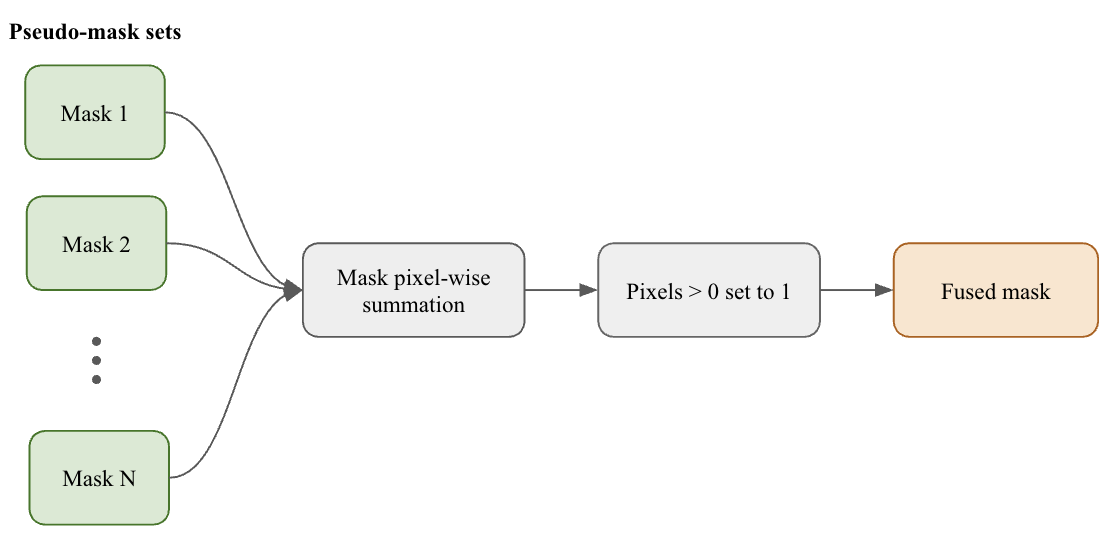
\includegraphics[width=\textwidth]{assets/images/for_presentation/dg-mask-fuse-2.png}
\par\end{centering}
\caption{The process of pseudo-masks fusion using quartile agreement levels
\label{fig:dg-mask-fuse-2}}
\end{figure}

\begin{figure}[H]
\begin{centering}
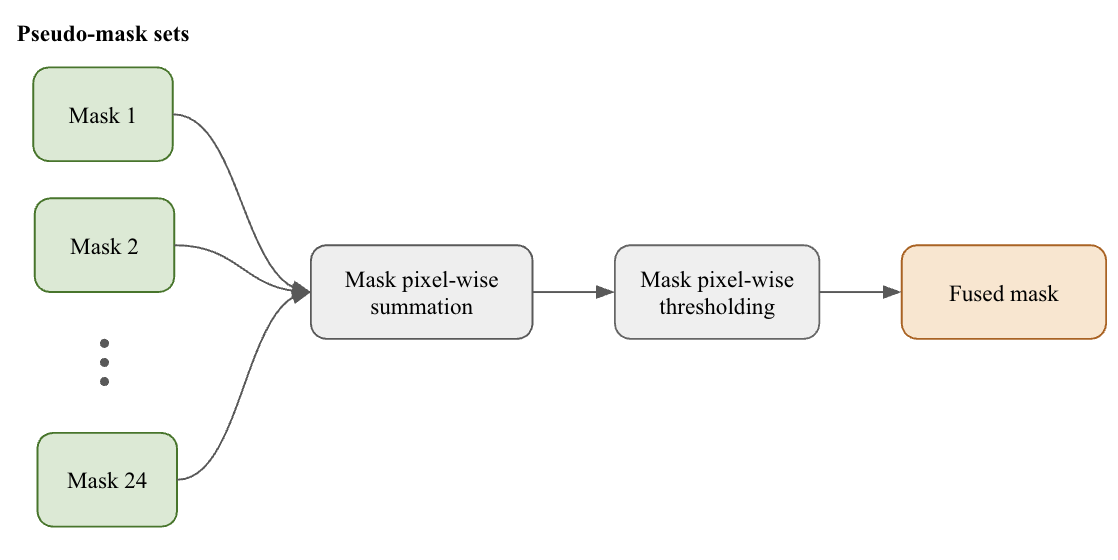
\includegraphics[width=\textwidth]{assets/images/for_presentation/dg-mask-fuse-1.png}
\par\end{centering}
\caption{The process of pseudo-masks fusing using voting consensus 
\label{fig:dg-mask-fuse-1}}
\end{figure}

\section{Experiments}
\label{section:experiments}
Our proposed system evolved with each performed experiment, since each experiment built on the previous one. We will describe each experiment in this section, with a focus on the data used for training and testing, the experiment setup and workflow, and the results of the experiment. Every experiment was run three times, to reduce the risk that random initialization of model's parameters, or the split of training data into training and validation subsets, would significantly improve or significantly worsen the final results.

For the first experiment, we utilized just the UNet model itself as a deep learning module. The fully annotated TNBC dataset was used for this task.

The second experiment used the pseudo-masks generated by a combination of image sources and different computer vision techniques. The pseudo-masks were generated for the weakly annotated TIGER dataset from the provided bounding box annotations.These were then used as ground truth masks for subsequent training of the U-Net model, which was trained on the TIGER dataset. For the final evaluation, the TNBC dataset was used.

The third experiment build on the second. It compared the different fusing strategies of mask sets. Again, we used these fused masks to train the U-Net model on the TIGER dataset, and the TNBC dataset was used for the final evaluation.

In the fourth experiment, we utilized a transfer learning strategy, where we took the best model trained during the third experiment and fine-tuned it using part of the fully annotated TNBC dataset.

\subsection{Experiment 1 - Training on Small Dataset with Full Annotations}
In the first experiment, we wanted to check whether the small, fully annotated TNBC dataset would be sufficient for training of the segmentation model.

\paragraph{Data}
We use only the fully annotated TNBC dataset, both for the training and for the final evaluation. This dataset is split into three folds, where the folds contain the following number of image patches:

\begin{itemize}
    \item Fold 1 contains 72 image patches, from 4 patients,
    \item Fold 2 contains 68 image patches, from 4 patients, and
    \item Fold 3 contains 60 image patches, from 3 patients
\end{itemize}

Always two folds were used as the training set and one fold was used as the testing set. Together this gave us three rounds of training and evaluation for one experiment run. To calculate the final result for each reported metric, the weighted average of the metrics logged by every round was calculated, given the Equation \ref{eq:weighted_avg}, where $\bar{M}$ is the final reported metric (Dice coefficient and IoU), $n$ is the number of the fold that was used for evaluation, $i$ is the \textit{i}-th fold used for model evaluation, $M_i$ is the evaluation metric calculated when evaluating the model on the \textit{i}-th fold, and $W_i$ is the size of the \textit{i}-th fold.

\begin{align}
\label{eq:weighted_avg}
\bar{M} &= \frac{\sum_{i=1}^{n} M_i \cdot W_i}{\sum_{i=1}^{n} W_i}
\end{align}

\paragraph{Experiment Workflow}
The workflow of this experiment is simple. We train the U-Net model using the TNBC dataset, with the provided ground truth masks and evaluate it on the same dataset.

\paragraph{Results}

\subsection{Experiment 2 - Pseudo-mask Generating Strategies}
\label{sub:exp-2}

\paragraph{Data}

\paragraph{Experiment Workflow}

\paragraph{Results}

\subsection{Experiment 3 - Pseudo-mask Fusing Strategies}

\paragraph{Data}

\paragraph{Experiment Workflow}

\paragraph{Results}

\subsection{Experiment 4 - Transfer Learning}

\paragraph{Data}

\paragraph{Experiment Workflow}

\paragraph{Results}

\subsection{Experiments Summary}

\section{Tools}
Python, 
NumPy, 
PyTorch, 
PyTorch Lightning,
Segmentation Models PyTorch, 
Torchstain multitarget macenko norm
Azure ml studio
Jupyter Notebooks
OpenCV
scikit-learn
Weights and Biases - For easier monitoring, logging, data visualization and the overall improved management of the whole training process, we use the Weights and Biases 
matplotlib.pyplot
PyCharm
Git
GitHub
CUDA